%-------------------------------------------------------------------------------
%-------------------------------------------------------------------------------
\begin{frame} I heavily draw on the material presented in:

\begin{itemize}
\item Whitney Newey, course materials for 14.385 Nonlinear Econometric Analysis, Fall 2007. MIT OpenCourseWare
(http://ocw.mit.edu), Massachusetts Institute of Technology.
\end{itemize}

\end{frame}
%-------------------------------------------------------------------------------
%-------------------------------------------------------------------------------
\begin{frame}\textbf{General idea}\vspace{0.3cm}
\begin{itemize}\setlength\itemsep{1em}
\item The generalized method of moments (GMM) is a general estimation principle, where the estimators are derived from so-called  moment conditions. It provides a unifying framework for the comparison of alternative estimators.
\end{itemize}

\end{frame}
%-------------------------------------------------------------------------------
%-------------------------------------------------------------------------------
\begin{frame}\textbf{Structure}\vspace{0.3cm}

\begin{itemize}\setlength\itemsep{1em}
\item Setup
\item Identification
\item Asymptotic theory
\item Testing
\end{itemize}
\end{frame}
%-------------------------------------------------------------------------------
%-------------------------------------------------------------------------------
\begin{frame}\textbf{Notation}\vspace{0.3cm}

\begin{itemize}\setlength\itemsep{1em}
\item $\beta$ denotes a $p \times 1$ parameter vector
\item $w_i$ is a data point with $i = 1, \hdots, n$
\item $g_i(\beta) = g(w_i, \beta)$ is a $m \times 1$ vector of functions of the data and parameters
\end{itemize}
\end{frame}
%-------------------------------------------------------------------------------
%-------------------------------------------------------------------------------
\begin{frame}

\begin{itemize}\setlength\itemsep{1em}
\item The GMM estimator is based on a model where, for the true parameter value $\beta_0$ the moment conditions
$E[g_i (\beta_0)] = 0$ are satisfied.
\item The estimator is formed by choosing $\beta$ so that the sample average of $g_i(\beta)$ is close to
its zero population value.
\end{itemize}

\end{frame}
%-------------------------------------------------------------------------------
%-------------------------------------------------------------------------------
\begin{frame}

The estimator is formed by choosing $\beta$ so that the sample average of $g_i(\beta)$ is close to its zero population value. Let

\begin{align*}
\hat{g}(\beta) = \frac{1}{n} \sum_{i=1}^n g_i(\beta)
\end{align*}

\begin{itemize}\setlength\itemsep{1em}
\item theoretical moments
\item empirical moments
\end{itemize}

\end{frame}
%-------------------------------------------------------------------------------
%-------------------------------------------------------------------------------
\begin{frame}
Let $\hat{A}$ denote a $m \times m$ positive semi-definite matrix, then the GMM estimator is given by

\begin{align*}
\hat{\beta} = \argmin_\beta \hat{g}(\beta)^\prime\,\hat{A}\,\hat{g}(\beta)
\end{align*}

The GMM estimator chooses $\hat{\beta}$ so the sample average $\hat{g}(\beta)$ is close to zero.

\end{frame}
%-------------------------------------------------------------------------------
%-------------------------------------------------------------------------------
\begin{frame}\textbf{Instrumental variables}\vspace{1cm}

\begin{center}
Let's work through an example on the blackboard.
\end{center}

\end{frame}
%-------------------------------------------------------------------------------
%-------------------------------------------------------------------------------
\begin{frame}\textbf{Unifying framework}\vspace{1cm}

Many other popular estimation strategies can be analyzed in a GMM setup.

\begin{align*}\begin{array}{ll}
\text{Ordinary least squares} & E[x_i (y_i - x_i \beta_0)] = 0 \\
\text{Instrumental variables} & E[z_i (y_i - x_i \beta_0)] = 0 \\
\text{Maximum likelihood}     & E[\partial \ln f(x_i, \beta_0) / \partial\beta] = 0
\end{array}
\end{align*}

\end{frame}
%-------------------------------------------------------------------------------
%-------------------------------------------------------------------------------
\begin{frame}

If moments cannot be evaluated analytically then we have an application of the method of simulated moments.
\end{frame}
%-------------------------------------------------------------------------------
%-------------------------------------------------------------------------------

\begin{frame}\textbf{Identification}\vspace{1cm}

The parameters $\beta_0$ are identified if $\beta_0$ is the only solution to  $E[g_i(\beta)] = 0$.

\end{frame}
%-------------------------------------------------------------------------------
%-------------------------------------------------------------------------------
\begin{frame}
\begin{figure}[htp]\centering
\scalebox{0.35}{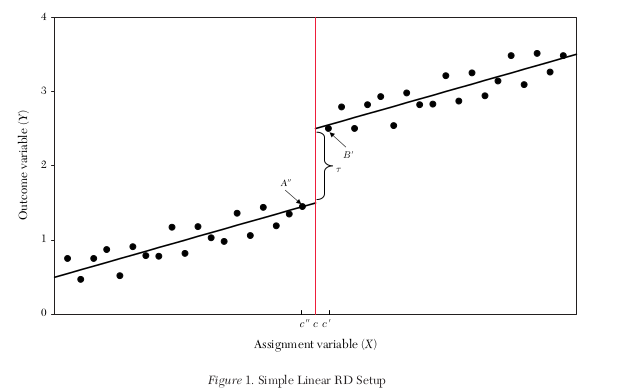
\includegraphics{material/figure-1}}
\end{figure}
\end{frame}

%-------------------------------------------------------------------------------
%-------------------------------------------------------------------------------
\begin{frame}

\begin{itemize}
\item Necessary condition for identification is that $m \geq p$. When $m \leq p$, i.e. there are fewer equations to solve than parameters, there will
typically be multiple solutions to the moment conditions.
\end{itemize}

\end{frame}
%-------------------------------------------------------------------------------
%-------------------------------------------------------------------------------
\begin{frame}

\begin{itemize}\setlength\itemsep{1em}
\item Let $G = E[\partial g_i(\beta_0) / \partial \beta]$. Rank condition is $rank(G) = p$. Necessary and sufficient for identification when $g_i(\beta)$ is linear in $\beta$.
\item In the general nonlinear case it is difficult to specify conditions for uniqueness of the solution to $E[g_i(\beta)] = 0$.
\end{itemize}

\end{frame}
%-------------------------------------------------------------------------------
%-------------------------------------------------------------------------------
\begin{frame}\textbf{Distance and weighing matrix}\vspace{0.3cm}

Let's look at the role of the weighing matrix for a two dimensional example.\vspace{0.3cm}

\begin{itemize}
\item identity matrix
\begin{align*}Q(\beta) =
\left(\begin{matrix}
g_1 & g_2
\end{matrix}\right)
\left(\begin{matrix}
1 & 0 \\
0 & 1
\end{matrix}\right)
\left(\begin{matrix}
g_1 \\
g_2
\end{matrix}\right) = g_1^2 + g_2^2
\end{align*}
\end{itemize}
\end{frame}
%-------------------------------------------------------------------------------
%-------------------------------------------------------------------------------
\begin{frame}

\begin{itemize}
\item alternative
\begin{align*}Q(\beta) =
\left(\begin{matrix}
g_1 & g_2
\end{matrix}\right)
\left(\begin{matrix}
2 & 0 \\
0 & 1
\end{matrix}\right)
\left(\begin{matrix}
g_1 \\
g_2
\end{matrix}\right) = 2 \dot g_1^2 + g_2^2
\end{align*}
\end{itemize}

Our alternative attaches more weight to the first coordinate in the distance.

\end{frame}
%-------------------------------------------------------------------------------
%-------------------------------------------------------------------------------
\begin{frame}\textbf{Asymptotic distribution}\vspace{0.3cm}

Under some regularity conditions, the GMM estimator has the following asymptotic distribution.

\begin{align*}
\sqrt{n}(\hat{\beta} - \beta_0) \xrightarrow{d} \N (0, V),
\end{align*}
where $V = (G^\prime A G)^{-1} G^\prime A \Omega A G (G^\prime A G)^{-1}$ with $G = E[\partial g_i(\beta_0) / \partial \beta]$ and $\Omega = E[g_i(\beta_0)g_i(\beta_0)^\prime]$.\\\vspace{0.3cm}

$\Rightarrow$ asymptotic variance depends on the choice of the weighing matrix $A$

\end{frame}
%-------------------------------------------------------------------------------
%-------------------------------------------------------------------------------
\begin{frame}

The optimal weighing matrix $A = \Omega^{-1}$ the asymptotic variance simplifies to

\begin{align*}
V = (G^\prime  \Omega^{-1} G)^{-1}\\
\end{align*}

What makes a good moment?
\begin{itemize}
\item small $S$, small sample variation of the moment
\item large $D$, moment informative on true value
\end{itemize}


\end{frame}
%-------------------------------------------------------------------------------
%-------------------------------------------------------------------------------
\begin{frame}\textbf{Instrumental variables}\vspace{1cm}

\begin{center}
Let's continue our example on the blackboard.
\end{center}

\end{frame}
%-------------------------------------------------------------------------------
%-------------------------------------------------------------------------------
\begin{frame}\textbf{Let's turn to our Jupyter notebooks ...}

\begin{figure}[htp]\centering
\scalebox{0.50}{
\includegraphics{material/jupyter}}
\end{figure}


\end{frame}
